\subsection{Proof of the implication ``strongly chordal  \texorpdfstring{$\Rightarrow$}{implies} MAT-free''}
\label{sub:if-part}
 
In this subsection we prove the ``if'' part of our main Theorem \ref{thm:MAT-free-strong-chordal} (strong chordality implies MAT-freeness). 
To find an MAT-labeling for a given strongly chordal graph, our strategy is to find compatible MAT-labelings of the subgraphs induced by all maximal cliques, then combine the constructions by the following ``gluing trick.''
\begin{theorem}[``Gluing trick'']
\label{glue}
Let $ G $ be a simple graph and suppose that $ V_{G} = A \cup B$, $E_{G} = E_{G[A]} \cup E_{G[B]} $, and $ A \cap B $ is a clique. 
Assume that there exist MAT-labelings $ \lambda_{A}, \lambda_{B}, \lambda_{A \cap B} $ of $ G[A], G[B], G[A\cap B] $, respectively  such that $ \lambda_{A}|_{E_{G[A\cap B]}} = \lambda_{B}|_{E_{G[A\cap B]}} =\lambda_{A\cap B}$. 
Define $ \lambda :=\lambda_{A} \cup \lambda_{B} \colon E_{G} \to \mathbb{Z}_{>0} $ by $\lambda|_A = \lambda_{A}, \lambda|_B = \lambda_{B}$, \ie 
\begin{align*}
\lambda(e) \coloneqq \begin{cases}
\lambda_{A}(e), & \text{ if } e \in E_{G[A]}, \\
\lambda_{B}(e), & \text{ if } e \in E_{G[B]}. 
\end{cases}
\end{align*}
\end{theorem}
\noindent
Then $ \lambda $ is an MAT-labeling of $ G $.
 
\begin{proof}
We proceed by induction on $ \ell = |V_{G}| $.
When $ \ell \leq 2 $ the assertion is trivial. 
Suppose $ \ell \geq 3 $. 
We may assume $ A \setminus  B \neq \varnothing $. 

We claim that $ G[A] $ has an MAT-simplicial vertex in $ A \setminus B $. 
First consider the case~$ A $ is a clique. 
Then any MAT-PEO of $ (G[A\cap B], \lambda_{A\cap B}) $ is extended to an MAT-PEO of $ (G[A], \lambda_{A}) $ by Lemma~\ref{MAT-L-PEO of complete graph}\ref{MAT-L-PEO of complete graph 1}, which shows the claim. 
Next suppose that $ A $ is not a clique. 
Then $ G[A] $ has two nonadjacent MAT-simplicial vertices by Lemma~\ref{lem:MATS-existence}\ref{MATS-existence 2}. 
At least one of them belongs to $ A \setminus B $ since $ A \cap B $ is a clique. 
Thus, in either case, $ G[A] $ has an MAT-simplicial vertex, say  $ v_{\ell} $ in $A \setminus B$.
Note that $ v_{\ell} $ is MAT-simplicial also in $ (G, \lambda) $ since $ N_{G}(v_{\ell}) \subseteq E_{G[A]} $. 

By Lemma \ref{MAT-simplicial}, $ \lambda_A|_{E_{G[A]\setminus v_{\ell}}} $ is an MAT-labeling. 
Consider the graph $ G\setminus v_{\ell} $ with the decomposition $ V_{G\setminus v_{\ell}} = (A\setminus \{v_{\ell}\}) \cup B $. 
By the induction hypothesis, we have that $ \lambda|_{E_{G \setminus v_{\ell}}} $ is an MAT-labeling. 
Using Lemma \ref{MAT-simplicial} again, we conclude that $ \lambda $ is an MAT-labeling of $G$. 
\end{proof}

The lemma below describes an important property (of antichains) of the clique intersection poset $ \mathcal{P}_{G} $.
\begin{lemma}\label{leaf}
Let $ G $ be a strongly chordal graph and let $ T \subseteq \mathcal{P}_{G} $ be an antichain with~$ |T| \geq 2 $.
Then there exist distinct $ X_{0}, Y_{0} \in T $ such that $ X_{0} \cap Y_{0} \supseteq X_{0} \cap Y $ for all $ Y \in T \setminus \{X_{0}\} $. 
\end{lemma}
\begin{proof}
Let $ Q $ be the subposet of $ \mathcal{P}_{G} $ induced by $  \Set{X \cap Y \in \mathcal{P}_{G} | X,Y \in T}  \supseteq T$. 
We will show that there exists a node $ X_{0} \in T $ such that $ X_{0} $ is a leaf of the Hasse diagram~$\mcH(Q)$ of $ Q $. 

Consider induced subposets of $ Q $ whose Hasse diagrams have the following form: 
\begin{center}
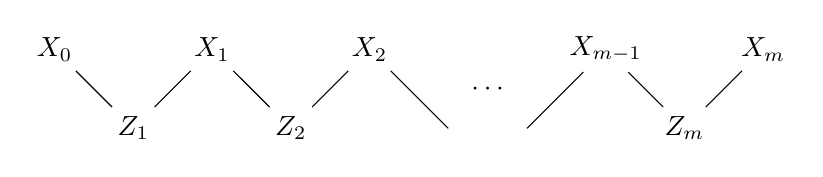
\begin{tikzpicture}[]
\node (X0) at (0,1) {$ X_{0} $};
\node (Z1) at (1,0) {$ Z_{1} $};
\node (X1) at (2,1) {$ X_{1} $};
\node (Z2) at (3,0) {$ Z_{2} $};
\node (X2) at (4,1) {$ X_{2} $};
\node (D) at (5.5,0.5) {$ \cdots $};
\node (Xm-1) at (7,1) {$ X_{m-1} $};
\node (Zm) at (8,0) {$ Z_{m} $};
\node (Xm) at (9,1) {$ X_{m} $};
\draw (X0)--(Z1)--(X1)--(Z2)--(X2)--(5,0);
\draw (6,0)--(Xm-1)--(Zm)--(Xm);
\end{tikzpicture}
\end{center}
where $ m \geq 0 $ and $ X_{i} \in T $ for all $ i \in \{0, \dots, m\} $.
Let $F= \{X_{0}, Z_{1}, \dots, Z_{m},X_{m}\} \subseteq Q $ be a poset of the form above such that $ m $ is maximum. 
Since the Hasse diagram does not change when we replace $ Z_{i} $ by $ X_{i-1} \cap X_{i} $ for each $ i \in \{1, \dots, m\} $, we may assume $ Z_{i} = X_{i-1} \cap X_{i} $. 

If $ X_{0} $ is not a leaf of $\mcH(Q)$, then there exists a node $ Z^{\prime} \in Q $ such that in $\mcH(Q)$,  $ Z^{\prime} $ is covered by $ X_{0} $ and the pair $ \{Z^{\prime}, Z_{1}\} $ is incomparable. 
Since every element in~$ Q\setminus T $ is the intersection of some elements in $ T $, there exists a node $ X^{\prime} \in T $ such that $ X^{\prime} \supsetneq Z^{\prime} $ and $ X^{\prime} \neq X_{0} $. 
Similarly, we may assume $ Z^{\prime} = X^{\prime} \cap X_{0} $. 

Since $ m $ is maximum, either $ X^{\prime} $ contains some $ Z_{j} \in F$, or $ Z^{\prime} $ is contained in some  $ X_{j} \in F \setminus \{X_0\}$. 
In either case, we obtain an induced subposet of $Q$ whose Hasse diagram has the form: 
\begin{center}
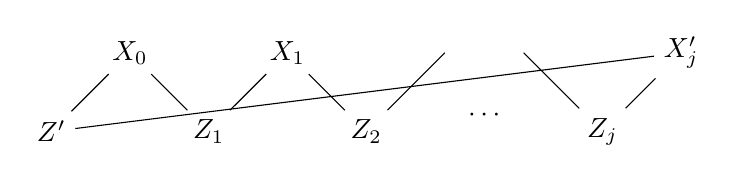
\begin{tikzpicture}[]
\node (Zp) at (0,0) {$ Z^{\prime} $};
\node (X0) at (1,1) {$ X_{0} $};
\node (Z1) at (2,0) {$ Z_{1} $};
\node (X1) at (3,1) {$ X_{1} $};
\node (Z2) at (4,0) {$ Z_{2} $};
\node (D) at (5.5,0.2) {$ \cdots $};
\node (Zj) at (7,0) {$ Z_{j} $};
\node (Xj) at (8,1) {$ X_{j}^{\prime} $};
\draw (Zp)--(X0)--(Z1)--(X1)--(Z2)--(5,1);
\draw (6,1)--(Zj)--(Xj)--(Zp); 
\end{tikzpicture}
\end{center}
where $ X_{j}^{\prime} $ denotes $ X_{j} $ or $ X^{\prime} $.

Since $ G $ is strongly chordal, $ \mathcal{P}_{G} $ is $ k $-crown-free for all $ k \geq 3 $ by Theorem \ref{Nevries-Rosenke}. 
Hence $ j = 1 $. 
Thus this leads to one of the following induced subposets: 
\begin{center}
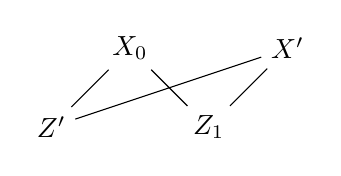
\begin{tikzpicture}[baseline=10]
\node (Zp) at (0,0) {$ Z^{\prime} $};
\node (X0) at (1,1) {$ X_{0} $};
\node (Z1) at (2,0) {$ Z_{1} $};
\node (Xp) at (3,1) {$ X^{\prime} $};
\draw (Zp)--(X0)--(Z1)--(Xp)--(Zp);
\end{tikzpicture}
\hspace{7mm} \hspace{7mm}
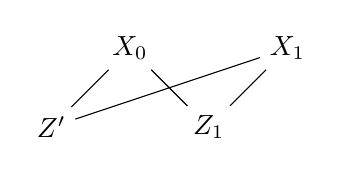
\begin{tikzpicture}[baseline=10]
\node (Zp) at (0,0) {$ Z^{\prime} $};
\node (X0) at (1,1) {$ X_{0} $};
\node (Z1) at (2,0) {$ Z_{1} $};
\node (X1) at (3,1) {$ X_{1} $};
\draw (Zp)--(X0)--(Z1)--(X1)--(Zp);
\end{tikzpicture}
\end{center}

If the first case occurs, then $ Z_{1} \subseteq X_{0} \cap X^{\prime} = Z^{\prime} $, which contradicts the incomparability of $ Z_{1} $ and $ Z^{\prime} $. 
When the second case occurs, $ Z^{\prime} \subseteq X_{0} \cap X_{1} = Z_{1} $, a contradiction again. 
In summary, $ X_{0} $ is a leaf of $\mcH(Q)$. 

Now let $ Y_{0} \cap Y_{1} \in Q$  for $Y_{0}, Y_{1} \in T$ denote a unique node in $ Q $ that is covered by~$ X_{0} $. 
We may assume that one of $Y_{0}, Y_{1}$ is not $X_0$, say $ Y_{0} \neq X_{0} $.
Then $ X_{0} \supsetneq X_{0} \cap Y_{0} \supseteq X_{0} \cap Y_{0} \cap Y_{1} = Y_{0} \cap Y_{1} $. 
Hence $ X_{0} \cap Y_{0} = Y_{0} \cap Y_{1} $. 

Finally let $ Y \in T\setminus\{X_{0}\} $. 
Then $ X_{0} \cap Y \in Q $ and $ X_{0} \cap Y \subsetneq X_{0} $. 
Since every path from $ X_{0} \cap Y $ to $ X_{0} $ passes through $   Y_{0} \cap Y_{1} $ in $\mcH(Q)$, we must have $ X_{0} \cap Y \subseteq X_{0} \cap Y_{0} $. 
\end{proof}
